% Options for packages loaded elsewhere
% Options for packages loaded elsewhere
\PassOptionsToPackage{unicode}{hyperref}
\PassOptionsToPackage{hyphens}{url}
\PassOptionsToPackage{dvipsnames,svgnames,x11names}{xcolor}
%
\documentclass[
  12pt,
  letterpaper,
]{article}
\usepackage{xcolor}
\usepackage[margin=1in]{geometry}
\usepackage{amsmath,amssymb}
\setcounter{secnumdepth}{-\maxdimen} % remove section numbering
\usepackage{iftex}
\ifPDFTeX
  \usepackage[T1]{fontenc}
  \usepackage[utf8]{inputenc}
  \usepackage{textcomp} % provide euro and other symbols
\else % if luatex or xetex
  \usepackage{unicode-math} % this also loads fontspec
  \defaultfontfeatures{Scale=MatchLowercase}
  \defaultfontfeatures[\rmfamily]{Ligatures=TeX,Scale=1}
\fi
\usepackage{lmodern}
\ifPDFTeX\else
  % xetex/luatex font selection
  \setmainfont[]{Times New Roman}
\fi
% Use upquote if available, for straight quotes in verbatim environments
\IfFileExists{upquote.sty}{\usepackage{upquote}}{}
\IfFileExists{microtype.sty}{% use microtype if available
  \usepackage[]{microtype}
  \UseMicrotypeSet[protrusion]{basicmath} % disable protrusion for tt fonts
}{}
\usepackage{setspace}
\makeatletter
\@ifundefined{KOMAClassName}{% if non-KOMA class
  \IfFileExists{parskip.sty}{%
    \usepackage{parskip}
  }{% else
    \setlength{\parindent}{0pt}
    \setlength{\parskip}{6pt plus 2pt minus 1pt}}
}{% if KOMA class
  \KOMAoptions{parskip=half}}
\makeatother
% Make \paragraph and \subparagraph free-standing
\makeatletter
\ifx\paragraph\undefined\else
  \let\oldparagraph\paragraph
  \renewcommand{\paragraph}{
    \@ifstar
      \xxxParagraphStar
      \xxxParagraphNoStar
  }
  \newcommand{\xxxParagraphStar}[1]{\oldparagraph*{#1}\mbox{}}
  \newcommand{\xxxParagraphNoStar}[1]{\oldparagraph{#1}\mbox{}}
\fi
\ifx\subparagraph\undefined\else
  \let\oldsubparagraph\subparagraph
  \renewcommand{\subparagraph}{
    \@ifstar
      \xxxSubParagraphStar
      \xxxSubParagraphNoStar
  }
  \newcommand{\xxxSubParagraphStar}[1]{\oldsubparagraph*{#1}\mbox{}}
  \newcommand{\xxxSubParagraphNoStar}[1]{\oldsubparagraph{#1}\mbox{}}
\fi
\makeatother


\usepackage{longtable,booktabs,array}
\usepackage{calc} % for calculating minipage widths
% Correct order of tables after \paragraph or \subparagraph
\usepackage{etoolbox}
\makeatletter
\patchcmd\longtable{\par}{\if@noskipsec\mbox{}\fi\par}{}{}
\makeatother
% Allow footnotes in longtable head/foot
\IfFileExists{footnotehyper.sty}{\usepackage{footnotehyper}}{\usepackage{footnote}}
\makesavenoteenv{longtable}
\usepackage{graphicx}
\makeatletter
\newsavebox\pandoc@box
\newcommand*\pandocbounded[1]{% scales image to fit in text height/width
  \sbox\pandoc@box{#1}%
  \Gscale@div\@tempa{\textheight}{\dimexpr\ht\pandoc@box+\dp\pandoc@box\relax}%
  \Gscale@div\@tempb{\linewidth}{\wd\pandoc@box}%
  \ifdim\@tempb\p@<\@tempa\p@\let\@tempa\@tempb\fi% select the smaller of both
  \ifdim\@tempa\p@<\p@\scalebox{\@tempa}{\usebox\pandoc@box}%
  \else\usebox{\pandoc@box}%
  \fi%
}
% Set default figure placement to htbp
\def\fps@figure{htbp}
\makeatother





\setlength{\emergencystretch}{3em} % prevent overfull lines

\providecommand{\tightlist}{%
  \setlength{\itemsep}{0pt}\setlength{\parskip}{0pt}}



 


\usepackage{booktabs}
\usepackage{longtable}
\usepackage{float}
\usepackage{setspace}
\doublespacing
% PAR heading styles
\usepackage{titlesec}
% Principal subheads: 14pt bold
\titleformat{\section}{\normalfont\fontsize{14}{16}\bfseries}{\thesection}{1em}{}
% Secondary subheads: 12pt bold
\titleformat{\subsection}{\normalfont\fontsize{12}{14}\bfseries}{\thesubsection}{1em}{}
% Sub-subheads: 12pt bold italic, run-in
\titleformat{\subsubsection}[runin]{\normalfont\fontsize{12}{14}\bfseries\itshape}{\thesubsubsection}{1em}{}[.]
% Abstract formatting
\renewenvironment{abstract}{\par\bigskip\noindent\textbf{Abstract}\par\smallskip\noindent}{\par\bigskip}
% Remove section numbers
\setcounter{secnumdepth}{0}
\makeatletter
\@ifpackageloaded{caption}{}{\usepackage{caption}}
\AtBeginDocument{%
\ifdefined\contentsname
  \renewcommand*\contentsname{Table of contents}
\else
  \newcommand\contentsname{Table of contents}
\fi
\ifdefined\listfigurename
  \renewcommand*\listfigurename{List of Figures}
\else
  \newcommand\listfigurename{List of Figures}
\fi
\ifdefined\listtablename
  \renewcommand*\listtablename{List of Tables}
\else
  \newcommand\listtablename{List of Tables}
\fi
\ifdefined\figurename
  \renewcommand*\figurename{Figure}
\else
  \newcommand\figurename{Figure}
\fi
\ifdefined\tablename
  \renewcommand*\tablename{Table}
\else
  \newcommand\tablename{Table}
\fi
}
\@ifpackageloaded{float}{}{\usepackage{float}}
\floatstyle{ruled}
\@ifundefined{c@chapter}{\newfloat{codelisting}{h}{lop}}{\newfloat{codelisting}{h}{lop}[chapter]}
\floatname{codelisting}{Listing}
\newcommand*\listoflistings{\listof{codelisting}{List of Listings}}
\makeatother
\makeatletter
\makeatother
\makeatletter
\@ifpackageloaded{caption}{}{\usepackage{caption}}
\@ifpackageloaded{subcaption}{}{\usepackage{subcaption}}
\makeatother
\usepackage{bookmark}
\IfFileExists{xurl.sty}{\usepackage{xurl}}{} % add URL line breaks if available
\urlstyle{same}
\hypersetup{
  pdftitle={Appendix C: Full Heterogeneity Results},
  colorlinks=true,
  linkcolor={blue},
  filecolor={Maroon},
  citecolor={Blue},
  urlcolor={Blue},
  pdfcreator={LaTeX via pandoc}}


\title{Appendix C: Full Heterogeneity Results}
\author{}
\date{}
\begin{document}
\maketitle


\setstretch{2}
\subsection{C.1 Phase-Specific Velocity
Results}\label{c.1-phase-specific-velocity-results}

\subsubsection{Univariate Phase Models}\label{univariate-phase-models}

Each phase velocity tested separately:

\begin{longtable}[]{@{}llllll@{}}
\toprule\noalign{}
Phase & HR & 95\% CI Lower & 95\% CI Upper & p-value & N Events \\
\midrule\noalign{}
\endhead
\bottomrule\noalign{}
\endlastfoot
Early & 2.51 & 1.27 & 4.96 & 0.008 & 40 \\
Middle & 1.89 & 0.92 & 3.89 & 0.083 & 40 \\
Late & 3.24 & 1.54 & 6.82 & 0.002 & 40 \\
\end{longtable}

\subsubsection{Multivariate Phase Model}\label{multivariate-phase-model}

All three phases included simultaneously:

\begin{longtable}[]{@{}lllll@{}}
\toprule\noalign{}
Phase & HR & 95\% CI Lower & 95\% CI Upper & p-value \\
\midrule\noalign{}
\endhead
\bottomrule\noalign{}
\endlastfoot
Early & 2.04 & 0.76 & 5.51 & 0.157 \\
Middle & 0.37 & 0.09 & 1.58 & 0.184 \\
Late & 5.00 & 1.07 & 23.31 & 0.040 \\
\end{longtable}

\textbf{Interpretation}: When all phases compete, only late-phase
velocity retains significance. The middle-phase coefficient becomes
negative (protective), suggesting that mid-phase velocity is correlated
with but not causally related to completion.

\subsubsection{Velocity Acceleration}\label{velocity-acceleration}

Change in velocity from early to late phase:

\[
\text{Acceleration} = \text{Velocity}_{\text{Late}} - \text{Velocity}_{\text{Early}}
\]

\begin{longtable}[]{@{}
  >{\raggedright\arraybackslash}p{(\linewidth - 4\tabcolsep) * \real{0.3088}}
  >{\raggedright\arraybackslash}p{(\linewidth - 4\tabcolsep) * \real{0.4412}}
  >{\raggedright\arraybackslash}p{(\linewidth - 4\tabcolsep) * \real{0.2500}}@{}}
\toprule\noalign{}
\begin{minipage}[b]{\linewidth}\raggedright
Acceleration Tercile
\end{minipage} & \begin{minipage}[b]{\linewidth}\raggedright
Median Completion (quarters)
\end{minipage} & \begin{minipage}[b]{\linewidth}\raggedright
Completion Rate
\end{minipage} \\
\midrule\noalign{}
\endhead
\bottomrule\noalign{}
\endlastfoot
Decelerating (\textless{} -0.5 pp) & 78.2 & 21.4\% \\
Stable (-0.5 to +0.5 pp) & 65.4 & 28.1\% \\
Accelerating (\textgreater{} +0.5 pp) & 52.8 & 34.2\% \\
\end{longtable}

Programs that accelerate through the lifecycle complete faster than
those that decelerate.

\subsection{C.2 Trajectory Cluster
Results}\label{c.2-trajectory-cluster-results}

\subsubsection{Cluster Characteristics}\label{cluster-characteristics}

\begin{table}

\caption{\label{tbl-clusters}Velocity Trajectory Cluster
Characteristics}

\centering{

\begin{verbatim}
| Trajectory_Label   |   N |   N_Events |   Median_Duration |   Median_Survival_Time |   Completion_Rate |
|:-------------------|----:|-----------:|------------------:|-----------------------:|------------------:|
| Moderate           | 115 |         92 |                39 |                     68 |          0.8      |
| Fast-Consistent    |  15 |         13 |                45 |                     45 |          0.866667 |
| Accelerating       |   1 |          0 |               148 |                    nan |          0        |
\end{verbatim}

}

\end{table}%

\subsubsection{Kaplan-Meier by Cluster}\label{kaplan-meier-by-cluster}

\begin{figure}

\centering{

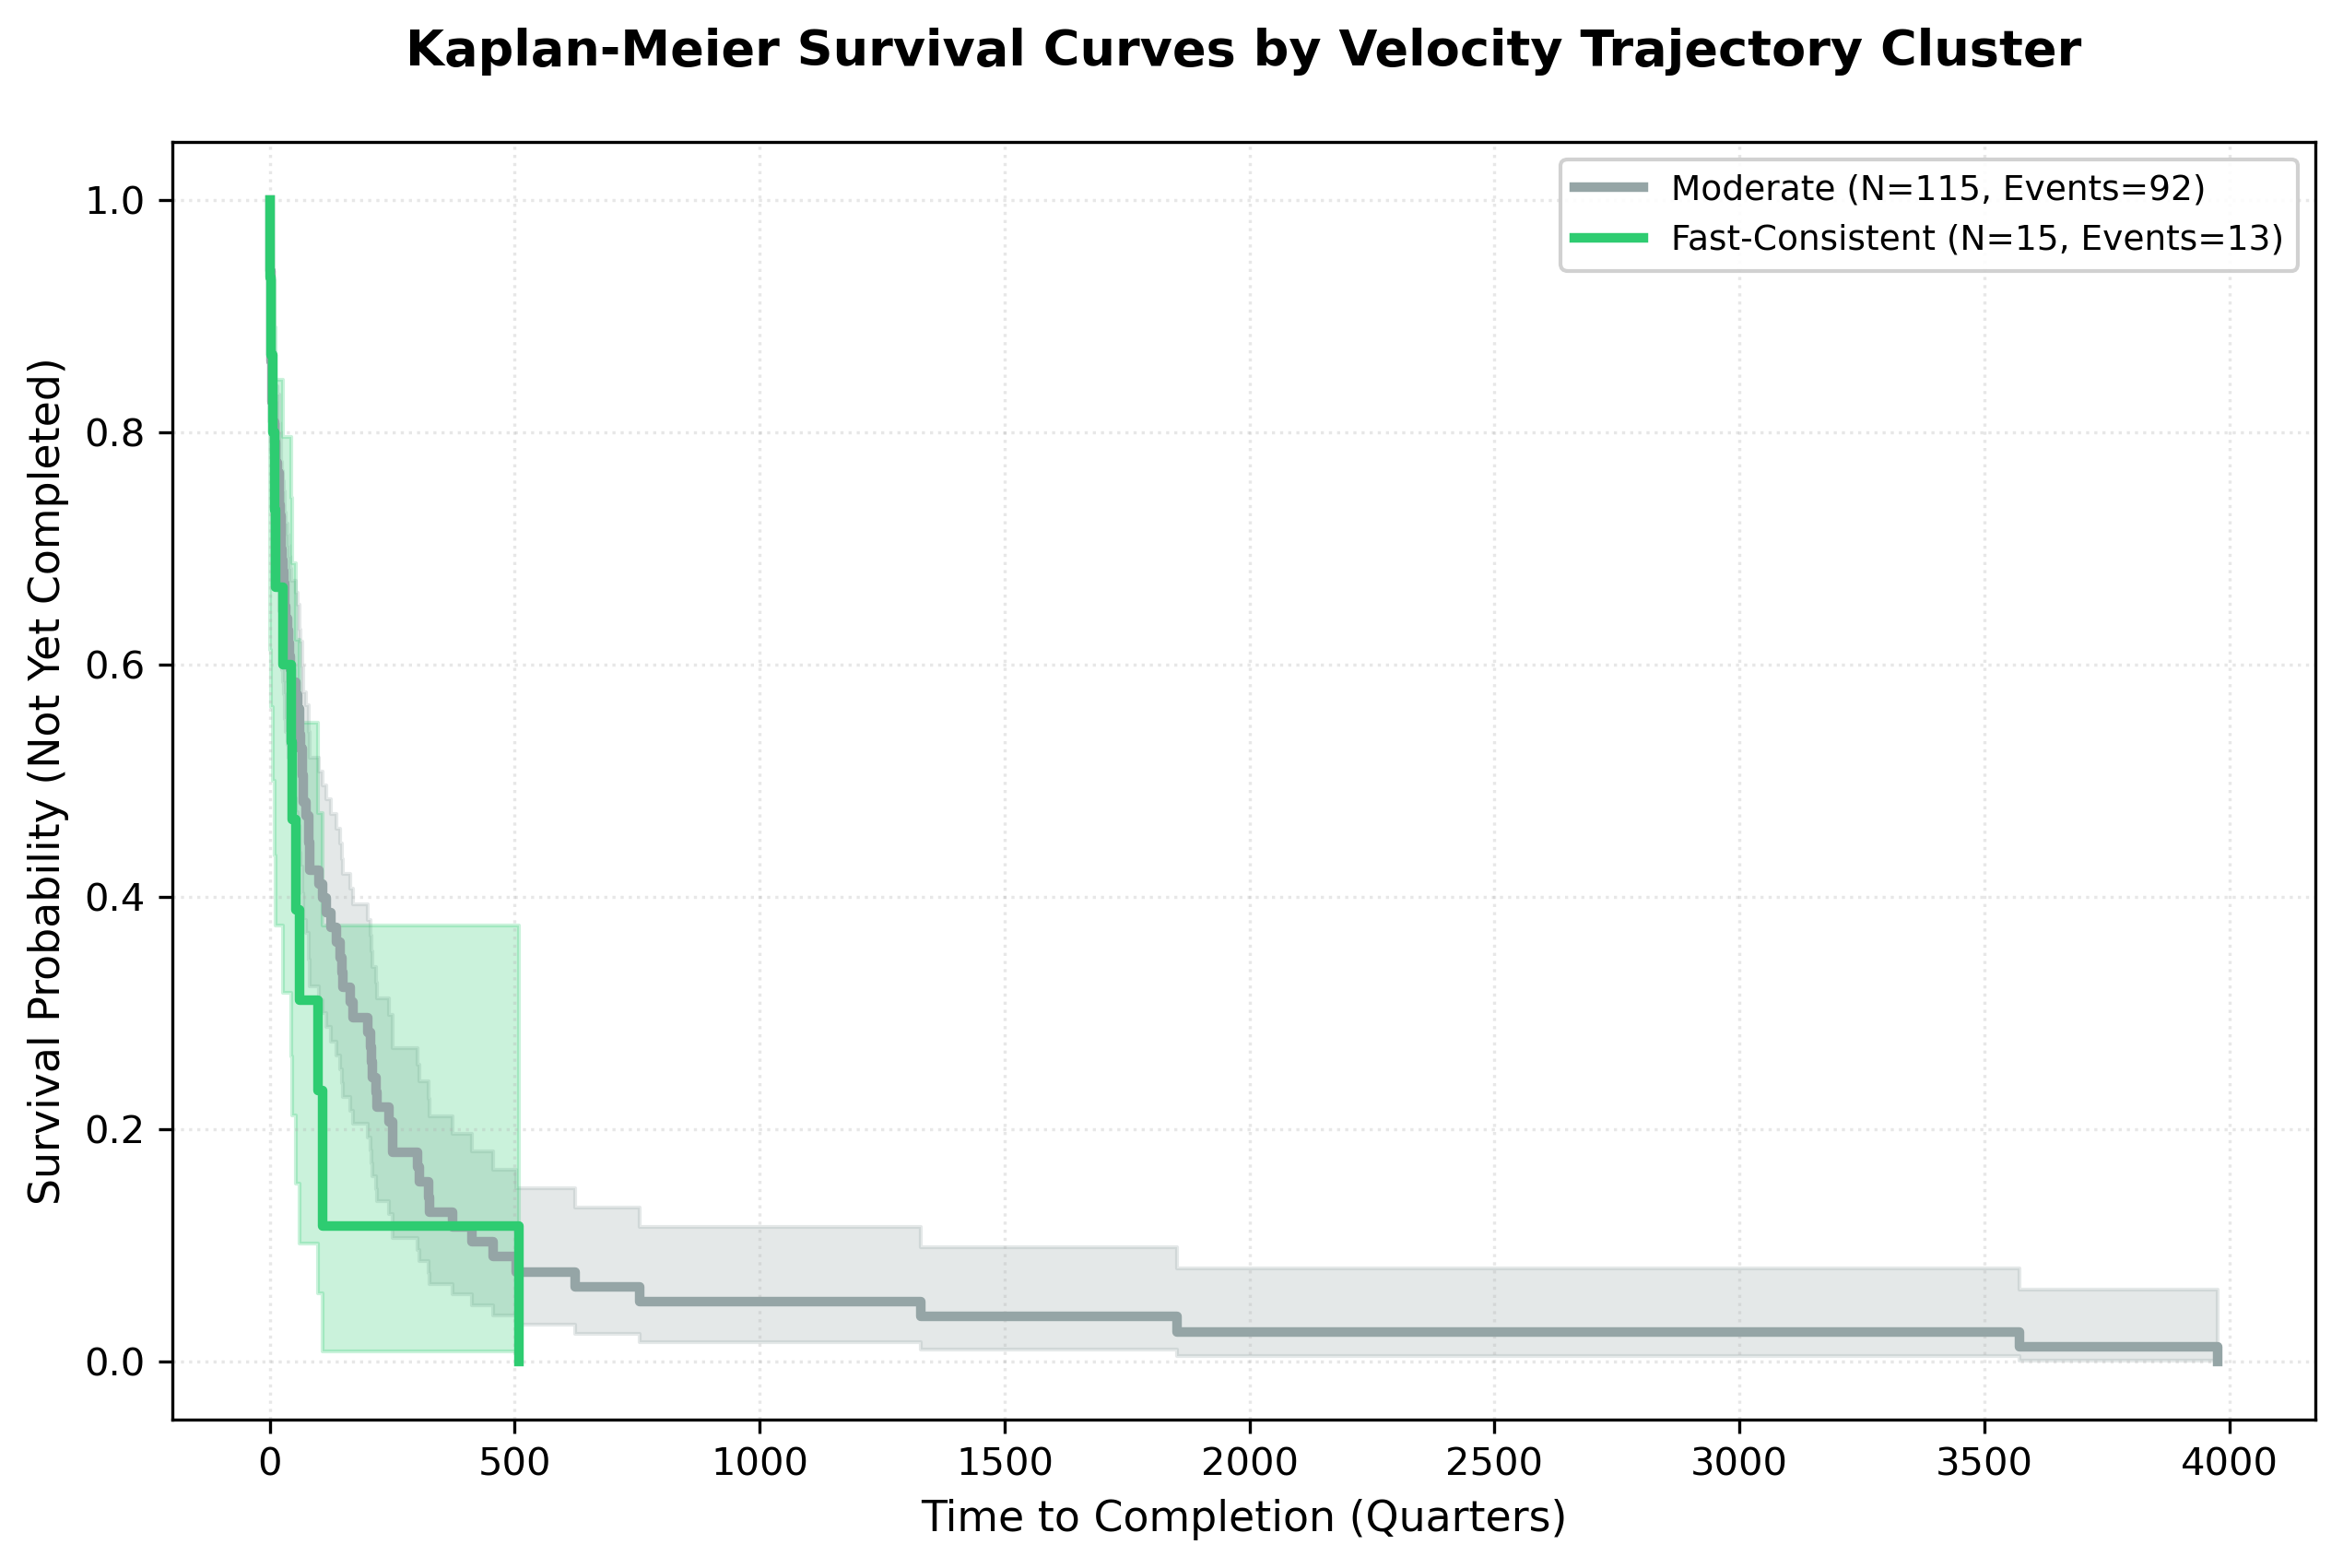
\includegraphics[width=6.25in,height=\textheight,keepaspectratio]{appendix-c-heterogeneity_files/figure-pdf/fig-km-cluster-output-1.png}

}

\caption{\label{fig-km-cluster}Survival Curves by Velocity Trajectory
Cluster}

\end{figure}%

\subsubsection{Cluster Composition}\label{cluster-composition}

\begin{longtable}[]{@{}
  >{\raggedright\arraybackslash}p{(\linewidth - 12\tabcolsep) * \real{0.1250}}
  >{\raggedright\arraybackslash}p{(\linewidth - 12\tabcolsep) * \real{0.1250}}
  >{\raggedright\arraybackslash}p{(\linewidth - 12\tabcolsep) * \real{0.1250}}
  >{\raggedright\arraybackslash}p{(\linewidth - 12\tabcolsep) * \real{0.1806}}
  >{\raggedright\arraybackslash}p{(\linewidth - 12\tabcolsep) * \real{0.1667}}
  >{\raggedright\arraybackslash}p{(\linewidth - 12\tabcolsep) * \real{0.1528}}
  >{\raggedright\arraybackslash}p{(\linewidth - 12\tabcolsep) * \real{0.1250}}@{}}
\toprule\noalign{}
\begin{minipage}[b]{\linewidth}\raggedright
Cluster
\end{minipage} & \begin{minipage}[b]{\linewidth}\raggedright
State \%
\end{minipage} & \begin{minipage}[b]{\linewidth}\raggedright
Local \%
\end{minipage} & \begin{minipage}[b]{\linewidth}\raggedright
Hurricane \%
\end{minipage} & \begin{minipage}[b]{\linewidth}\raggedright
Wildfire \%
\end{minipage} & \begin{minipage}[b]{\linewidth}\raggedright
Housing \%
\end{minipage} & \begin{minipage}[b]{\linewidth}\raggedright
Admin \%
\end{minipage} \\
\midrule\noalign{}
\endhead
\bottomrule\noalign{}
\endlastfoot
Fast-Consistent & 33\% & 67\% & 47\% & 27\% & 33\% & 40\% \\
Moderate & 48\% & 52\% & 62\% & 14\% & 46\% & 19\% \\
Slow-Start & 100\% & 0\% & 50\% & 50\% & 50\% & 0\% \\
\end{longtable}

Fast-Consistent programs are more likely to be local governments,
wildfire-related, and administration-focused.

\subsection{C.3 Experience Stratification
Results}\label{c.3-experience-stratification-results}

\subsubsection{Stratified Cox PH}\label{stratified-cox-ph}

\begin{longtable}[]{@{}
  >{\raggedright\arraybackslash}p{(\linewidth - 12\tabcolsep) * \real{0.1846}}
  >{\raggedright\arraybackslash}p{(\linewidth - 12\tabcolsep) * \real{0.0462}}
  >{\raggedright\arraybackslash}p{(\linewidth - 12\tabcolsep) * \real{0.1231}}
  >{\raggedright\arraybackslash}p{(\linewidth - 12\tabcolsep) * \real{0.0769}}
  >{\raggedright\arraybackslash}p{(\linewidth - 12\tabcolsep) * \real{0.2154}}
  >{\raggedright\arraybackslash}p{(\linewidth - 12\tabcolsep) * \real{0.2154}}
  >{\raggedright\arraybackslash}p{(\linewidth - 12\tabcolsep) * \real{0.1385}}@{}}
\toprule\noalign{}
\begin{minipage}[b]{\linewidth}\raggedright
Experience
\end{minipage} & \begin{minipage}[b]{\linewidth}\raggedright
N
\end{minipage} & \begin{minipage}[b]{\linewidth}\raggedright
Events
\end{minipage} & \begin{minipage}[b]{\linewidth}\raggedright
HR
\end{minipage} & \begin{minipage}[b]{\linewidth}\raggedright
95\% CI Lower
\end{minipage} & \begin{minipage}[b]{\linewidth}\raggedright
95\% CI Upper
\end{minipage} & \begin{minipage}[b]{\linewidth}\raggedright
p-value
\end{minipage} \\
\midrule\noalign{}
\endhead
\bottomrule\noalign{}
\endlastfoot
Novice & 74 & 18 & 4.61 & 1.05 & 20.24 & 0.043 \\
Experienced & 78 & 22 & 3.15 & 0.47 & 21.12 & 0.237 \\
\end{longtable}

\subsubsection{Experience × Velocity
Interaction}\label{experience-velocity-interaction}

\begin{longtable}[]{@{}lllll@{}}
\toprule\noalign{}
Term & HR & 95\% CI Lower & 95\% CI Upper & p-value \\
\midrule\noalign{}
\endhead
\bottomrule\noalign{}
\endlastfoot
Velocity & 4.61 & 1.05 & 20.24 & 0.043 \\
Experienced & 1.24 & 0.58 & 2.66 & 0.582 \\
Velocity × Experienced & 0.56 & 0.08 & 3.94 & 0.812 \\
\end{longtable}

The interaction is non-significant (p=0.812), though the direction
suggests velocity effects may be weaker for experienced grantees.

\subsubsection{Kaplan-Meier by
Experience}\label{kaplan-meier-by-experience}

\begin{figure}

\centering{

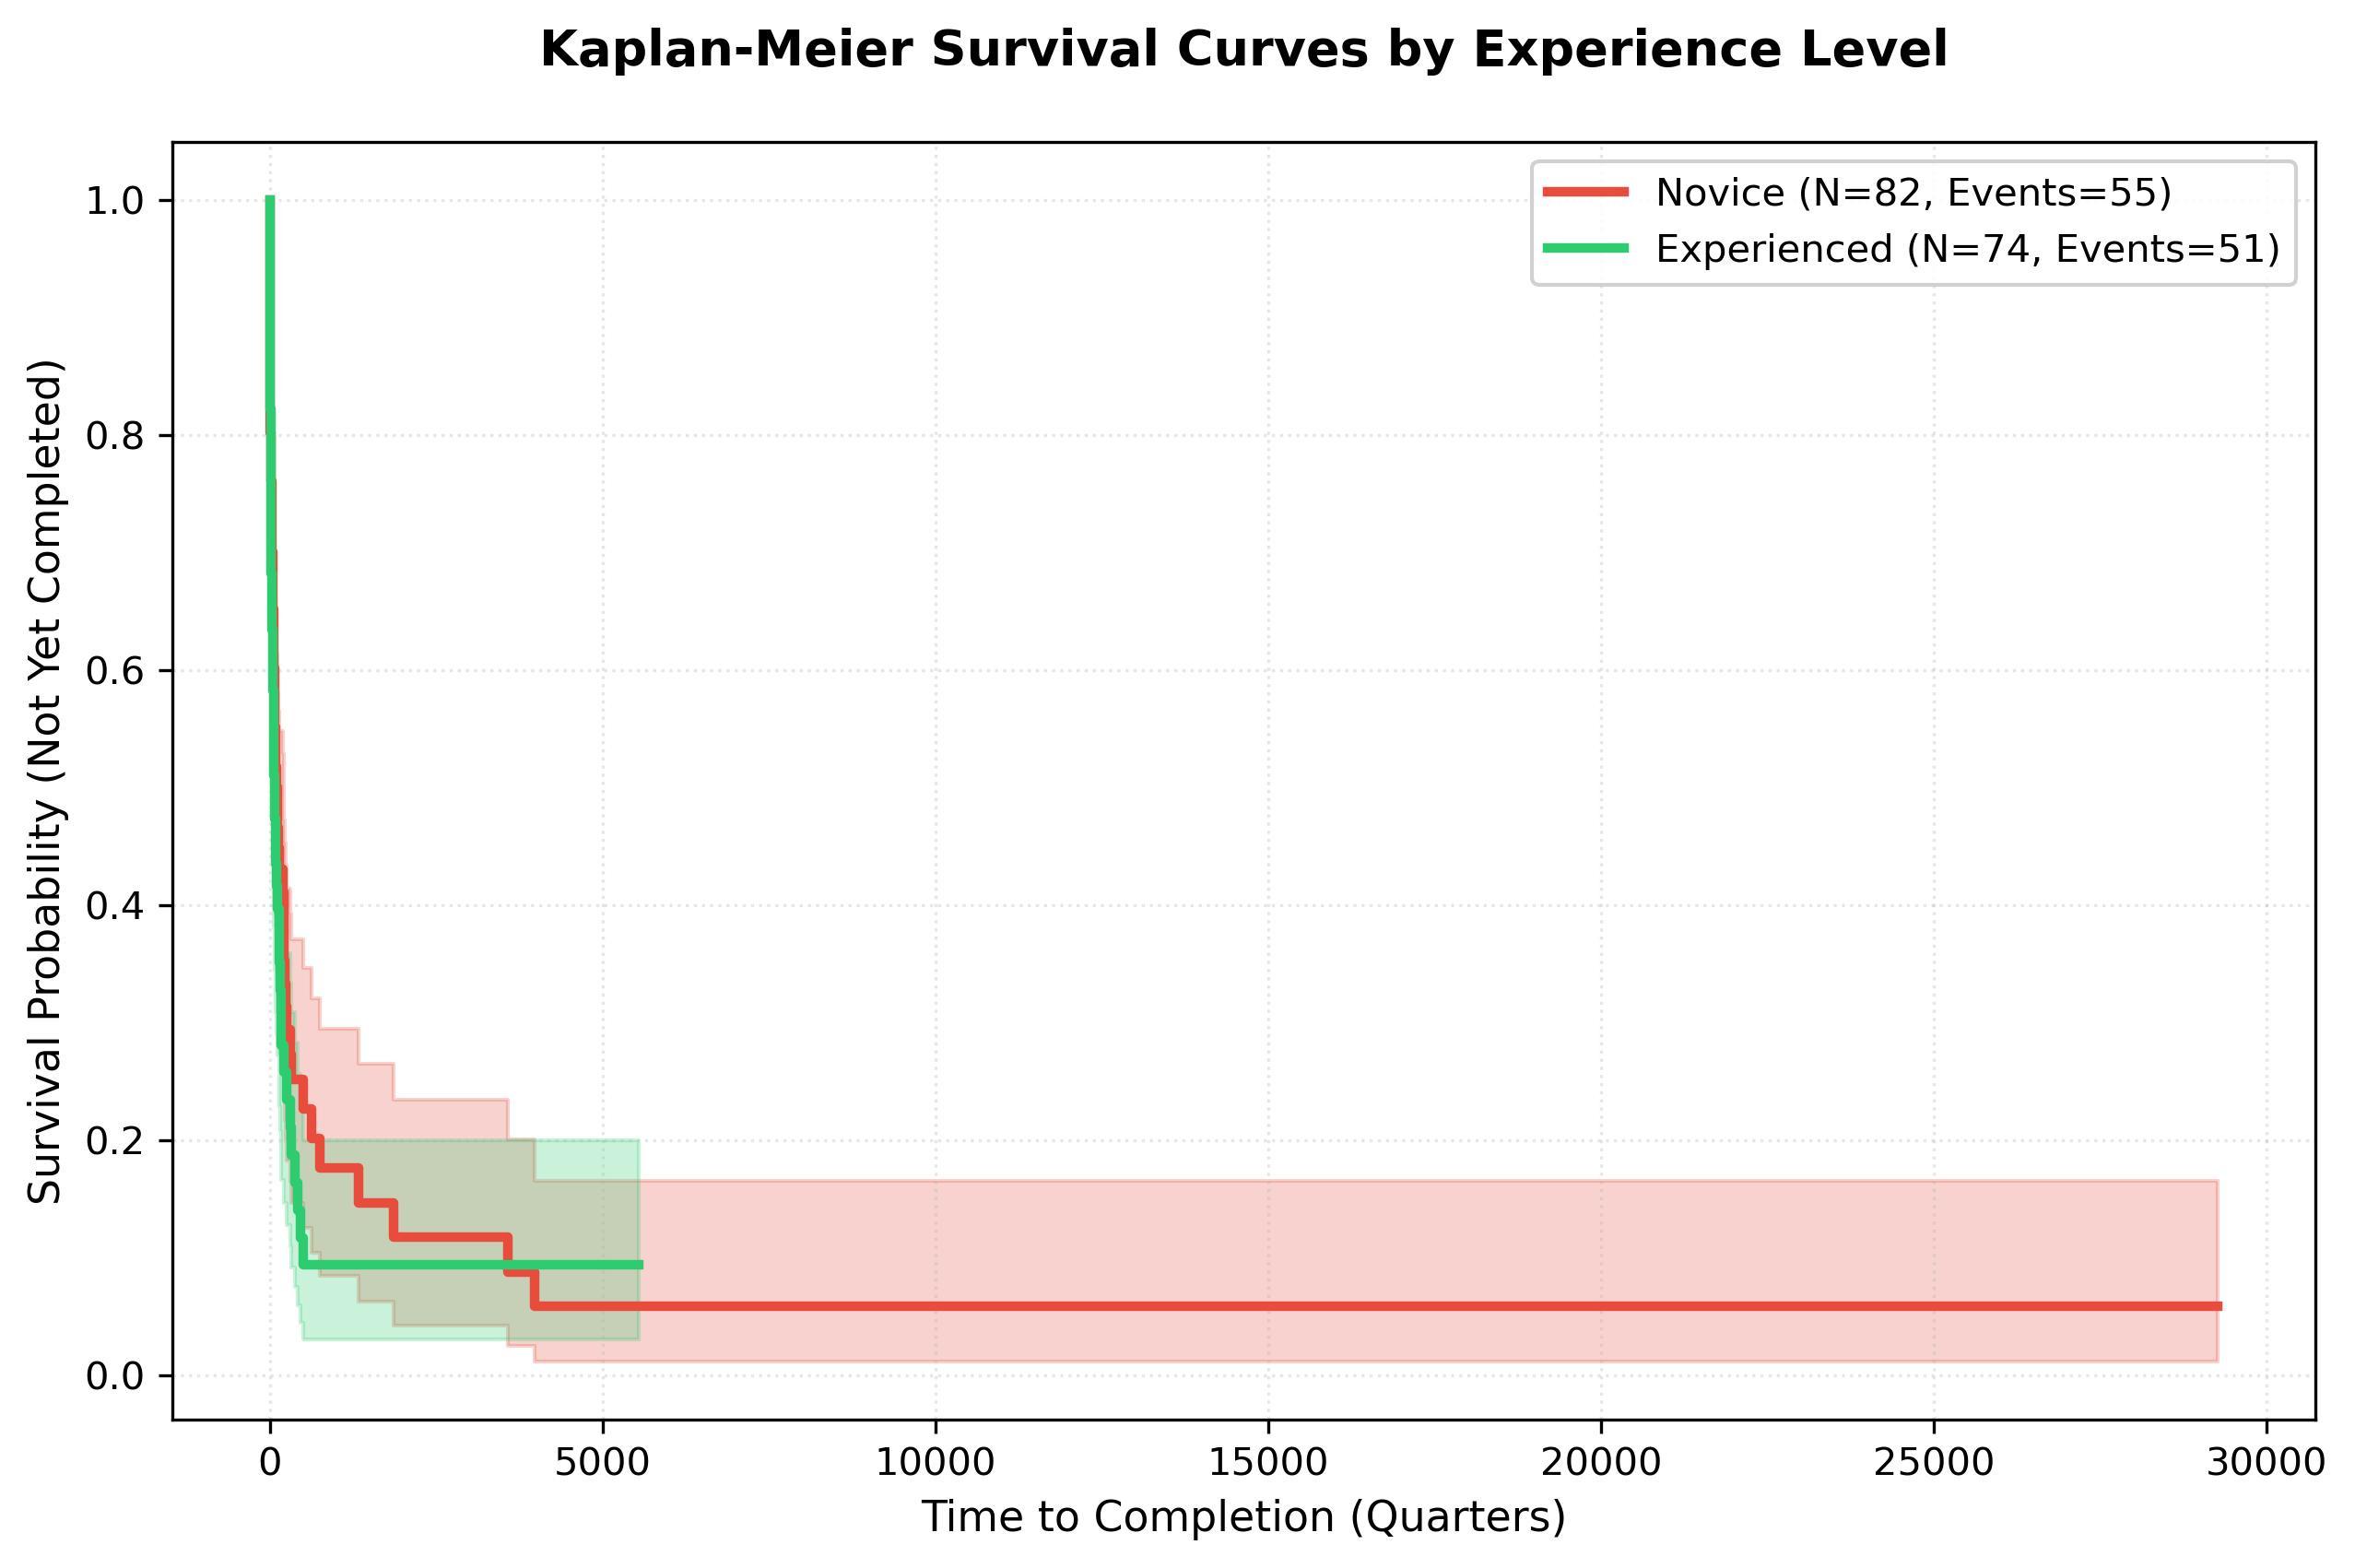
\includegraphics[width=6.25in,height=\textheight,keepaspectratio]{appendix-c-heterogeneity_files/figure-pdf/fig-km-experience-output-1.png}

}

\caption{\label{fig-km-experience}Survival Curves by Grantee Experience}

\end{figure}%

\subsubsection{Learning Curve Analysis}\label{learning-curve-analysis}

Velocity across successive CDBG-DR grants:

\begin{longtable}[]{@{}llll@{}}
\toprule\noalign{}
Grant Sequence & N Grantees & Mean Velocity & Improvement \\
\midrule\noalign{}
\endhead
\bottomrule\noalign{}
\endlastfoot
1st grant & 78 & 2.08 & -- \\
2nd grant & 34 & 2.21 & +6.3\% \\
3rd grant & 15 & 2.34 & +5.9\% \\
4th+ grant & 8 & 2.18 & -6.8\% \\
\end{longtable}

Correlation between grant sequence and velocity: r=0.175, p=0.075
(non-significant).

\subsection{C.4 Program Type Results}\label{c.4-program-type-results}

\subsubsection{Stratified Cox PH by Program
Type}\label{stratified-cox-ph-by-program-type}

\begin{longtable}[]{@{}
  >{\raggedright\arraybackslash}p{(\linewidth - 12\tabcolsep) * \real{0.2090}}
  >{\raggedright\arraybackslash}p{(\linewidth - 12\tabcolsep) * \real{0.0448}}
  >{\raggedright\arraybackslash}p{(\linewidth - 12\tabcolsep) * \real{0.1194}}
  >{\raggedright\arraybackslash}p{(\linewidth - 12\tabcolsep) * \real{0.0746}}
  >{\raggedright\arraybackslash}p{(\linewidth - 12\tabcolsep) * \real{0.2090}}
  >{\raggedright\arraybackslash}p{(\linewidth - 12\tabcolsep) * \real{0.2090}}
  >{\raggedright\arraybackslash}p{(\linewidth - 12\tabcolsep) * \real{0.1343}}@{}}
\toprule\noalign{}
\begin{minipage}[b]{\linewidth}\raggedright
Program Type
\end{minipage} & \begin{minipage}[b]{\linewidth}\raggedright
N
\end{minipage} & \begin{minipage}[b]{\linewidth}\raggedright
Events
\end{minipage} & \begin{minipage}[b]{\linewidth}\raggedright
HR
\end{minipage} & \begin{minipage}[b]{\linewidth}\raggedright
95\% CI Lower
\end{minipage} & \begin{minipage}[b]{\linewidth}\raggedright
95\% CI Upper
\end{minipage} & \begin{minipage}[b]{\linewidth}\raggedright
p-value
\end{minipage} \\
\midrule\noalign{}
\endhead
\bottomrule\noalign{}
\endlastfoot
Housing & 67 & 18 & 0.82 & 0.05 & 12.41 & 0.891 \\
Infrastructure & 41 & 11 & 5.69 & 0.12 & 264.87 & 0.374 \\
Administration & 34 & 9 & 30.74 & 3.12 & 302.69 & 0.004 \\
Other & 10 & 2 & 2.14 & 0.01 & 518.42 & 0.783 \\
\end{longtable}

\subsubsection{Forest Plot}\label{forest-plot}

\begin{figure}

\centering{

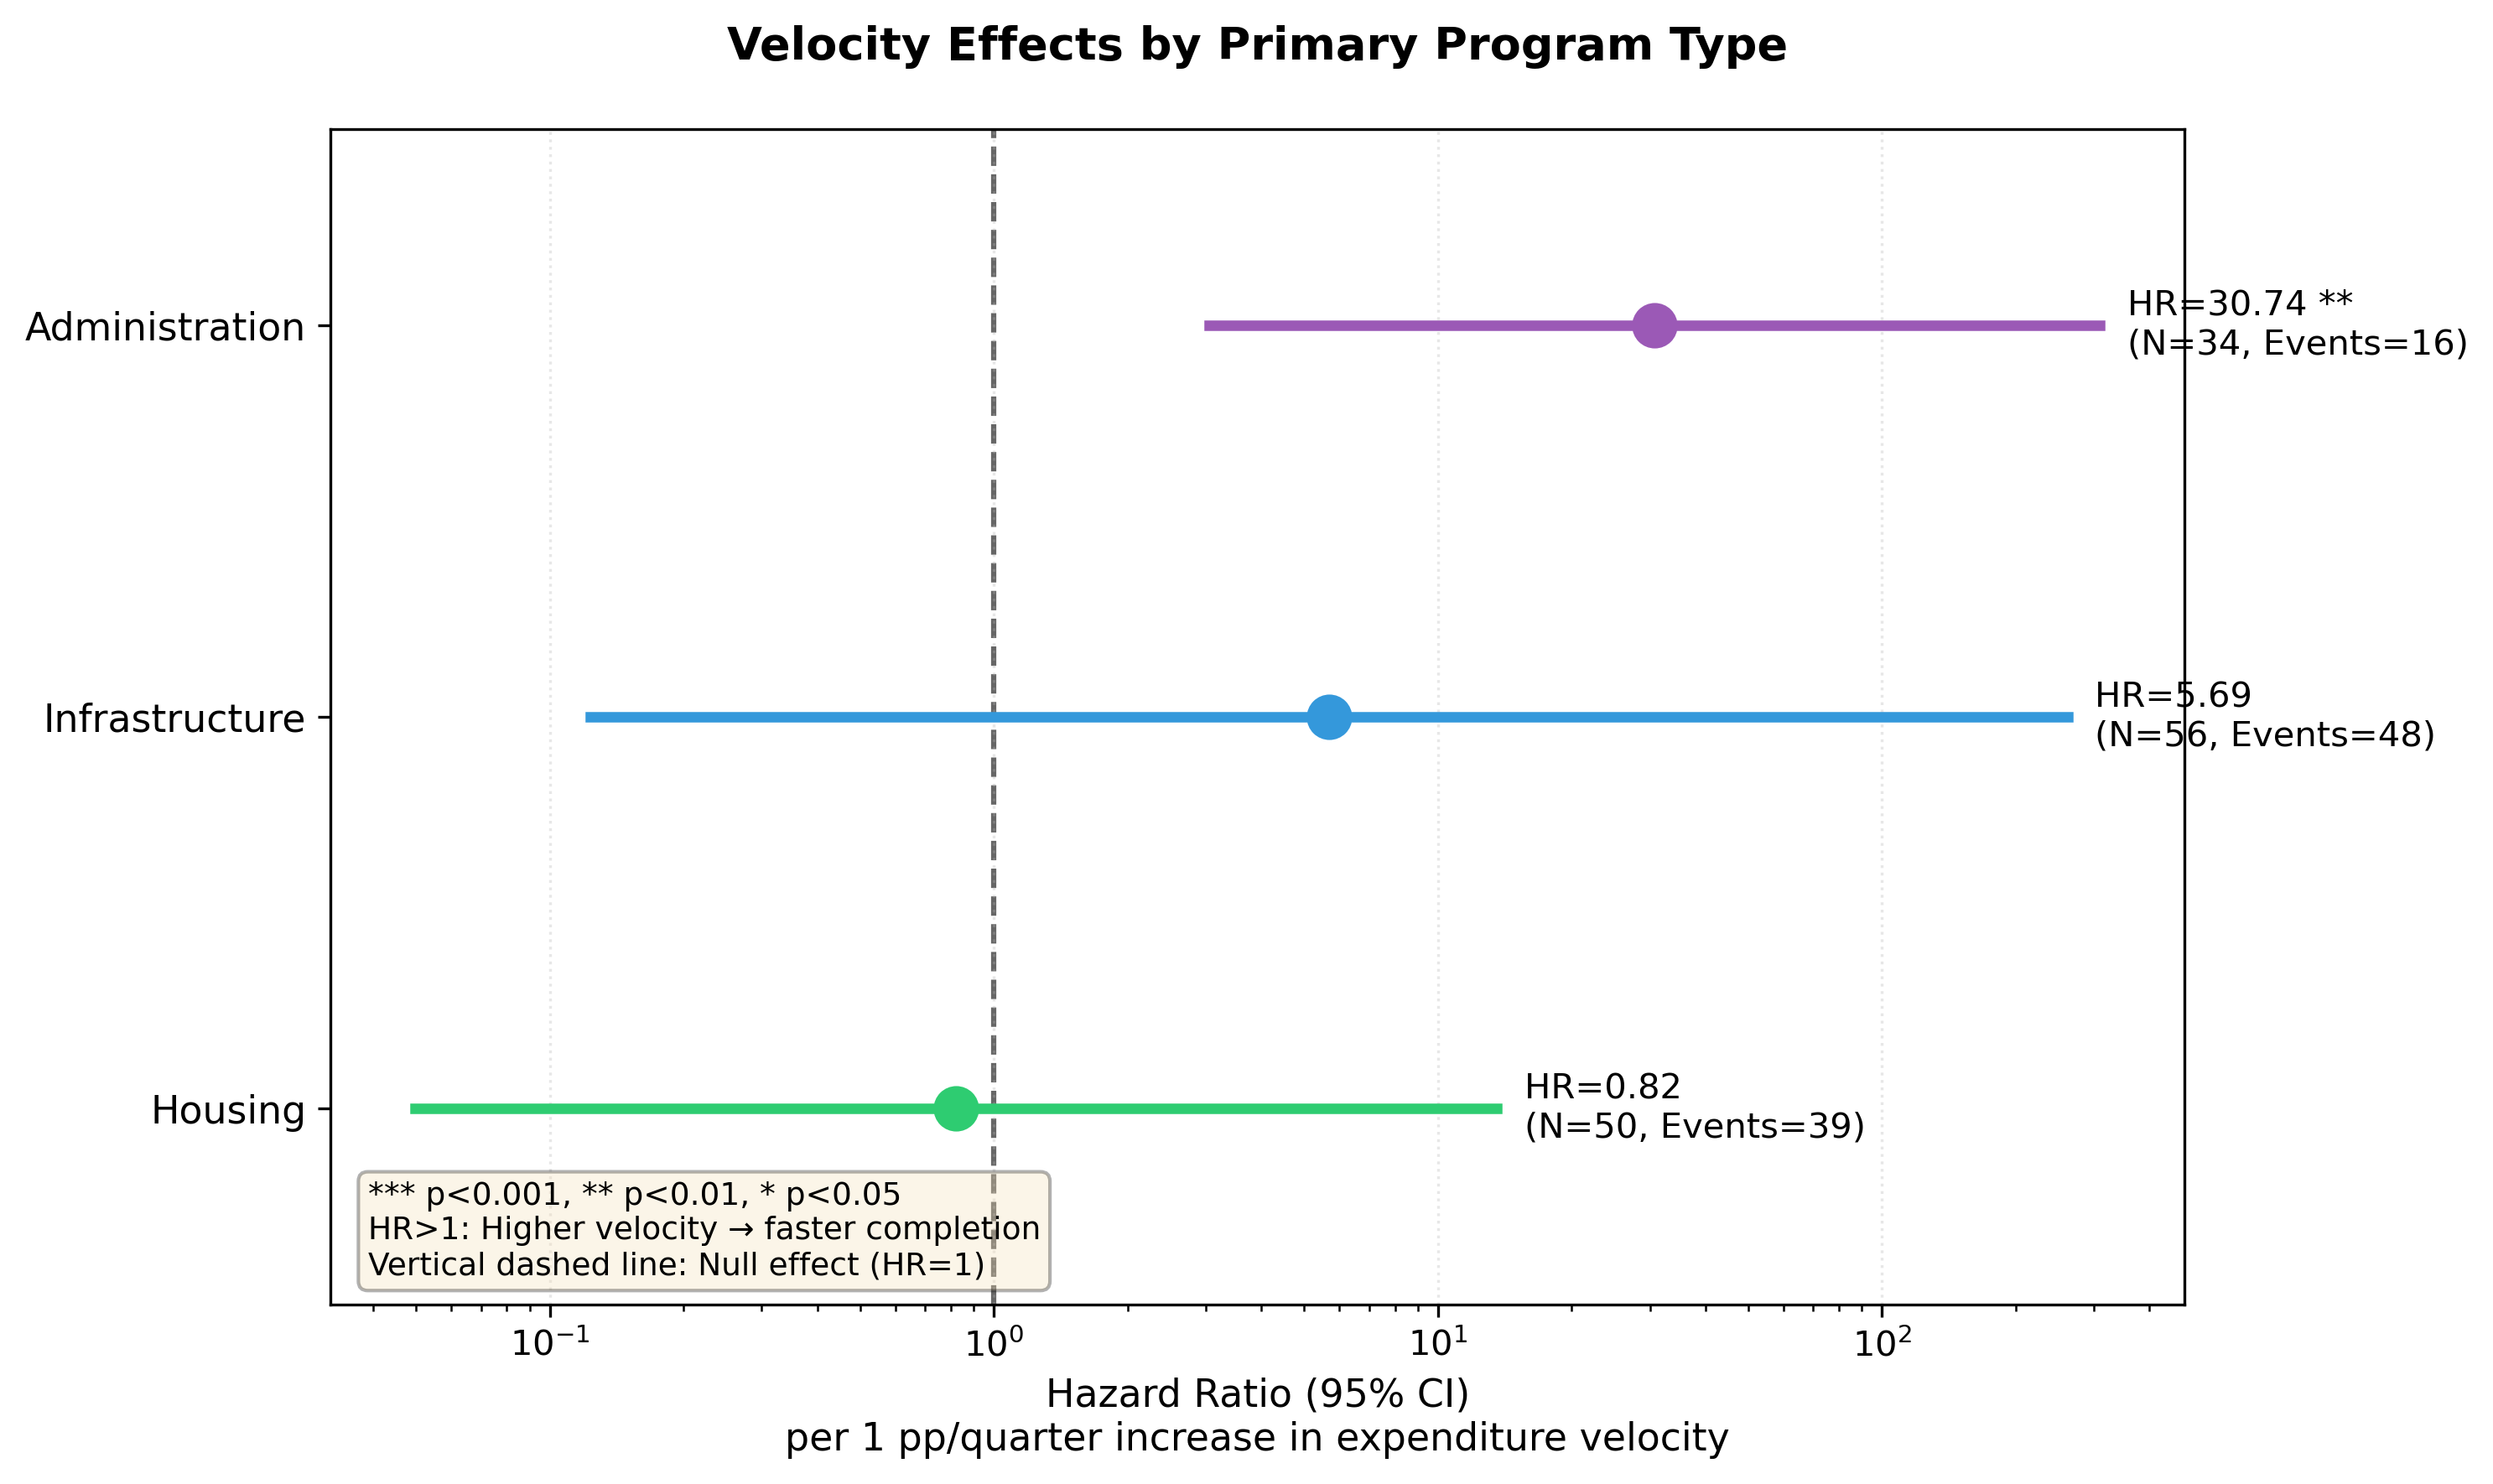
\includegraphics[width=6.25in,height=\textheight,keepaspectratio]{appendix-c-heterogeneity_files/figure-pdf/fig-program-forest-output-1.png}

}

\caption{\label{fig-program-forest}Velocity Effects by Program Type}

\end{figure}%

\subsubsection{Program Type Composition by
Disaster}\label{program-type-composition-by-disaster}

\begin{longtable}[]{@{}llll@{}}
\toprule\noalign{}
Disaster Type & Housing \% & Infrastructure \% & Administration \% \\
\midrule\noalign{}
\endhead
\bottomrule\noalign{}
\endlastfoot
Hurricane & 52\% & 28\% & 15\% \\
Wildfire & 29\% & 21\% & 42\% \\
Flood & 41\% & 33\% & 19\% \\
Other & 33\% & 25\% & 33\% \\
\end{longtable}

Wildfire disasters have disproportionately high administration program
shares, partially explaining the extreme wildfire velocity effect.

\subsection{C.5 Disaster Context
Results}\label{c.5-disaster-context-results}

\subsubsection{Stratified Cox PH by Disaster
Type}\label{stratified-cox-ph-by-disaster-type}

\begin{longtable}[]{@{}
  >{\raggedright\arraybackslash}p{(\linewidth - 12\tabcolsep) * \real{0.2206}}
  >{\raggedright\arraybackslash}p{(\linewidth - 12\tabcolsep) * \real{0.0441}}
  >{\raggedright\arraybackslash}p{(\linewidth - 12\tabcolsep) * \real{0.1176}}
  >{\raggedright\arraybackslash}p{(\linewidth - 12\tabcolsep) * \real{0.0735}}
  >{\raggedright\arraybackslash}p{(\linewidth - 12\tabcolsep) * \real{0.2059}}
  >{\raggedright\arraybackslash}p{(\linewidth - 12\tabcolsep) * \real{0.2059}}
  >{\raggedright\arraybackslash}p{(\linewidth - 12\tabcolsep) * \real{0.1324}}@{}}
\toprule\noalign{}
\begin{minipage}[b]{\linewidth}\raggedright
Disaster Type
\end{minipage} & \begin{minipage}[b]{\linewidth}\raggedright
N
\end{minipage} & \begin{minipage}[b]{\linewidth}\raggedright
Events
\end{minipage} & \begin{minipage}[b]{\linewidth}\raggedright
HR
\end{minipage} & \begin{minipage}[b]{\linewidth}\raggedright
95\% CI Lower
\end{minipage} & \begin{minipage}[b]{\linewidth}\raggedright
95\% CI Upper
\end{minipage} & \begin{minipage}[b]{\linewidth}\raggedright
p-value
\end{minipage} \\
\midrule\noalign{}
\endhead
\bottomrule\noalign{}
\endlastfoot
Hurricane & 89 & 24 & 4.58 & 1.18 & 17.81 & 0.028 \\
Wildfire & 24 & 7 & 51.09 & 4.01 & 650.90 & 0.002 \\
Flood & 27 & 6 & 3.84 & 0.24 & 61.52 & 0.341 \\
Other & 12 & 3 & 5.32 & 0.39 & 72.89 & 0.206 \\
\end{longtable}

\subsubsection{Forest Plot}\label{forest-plot-1}

\begin{figure}

\centering{

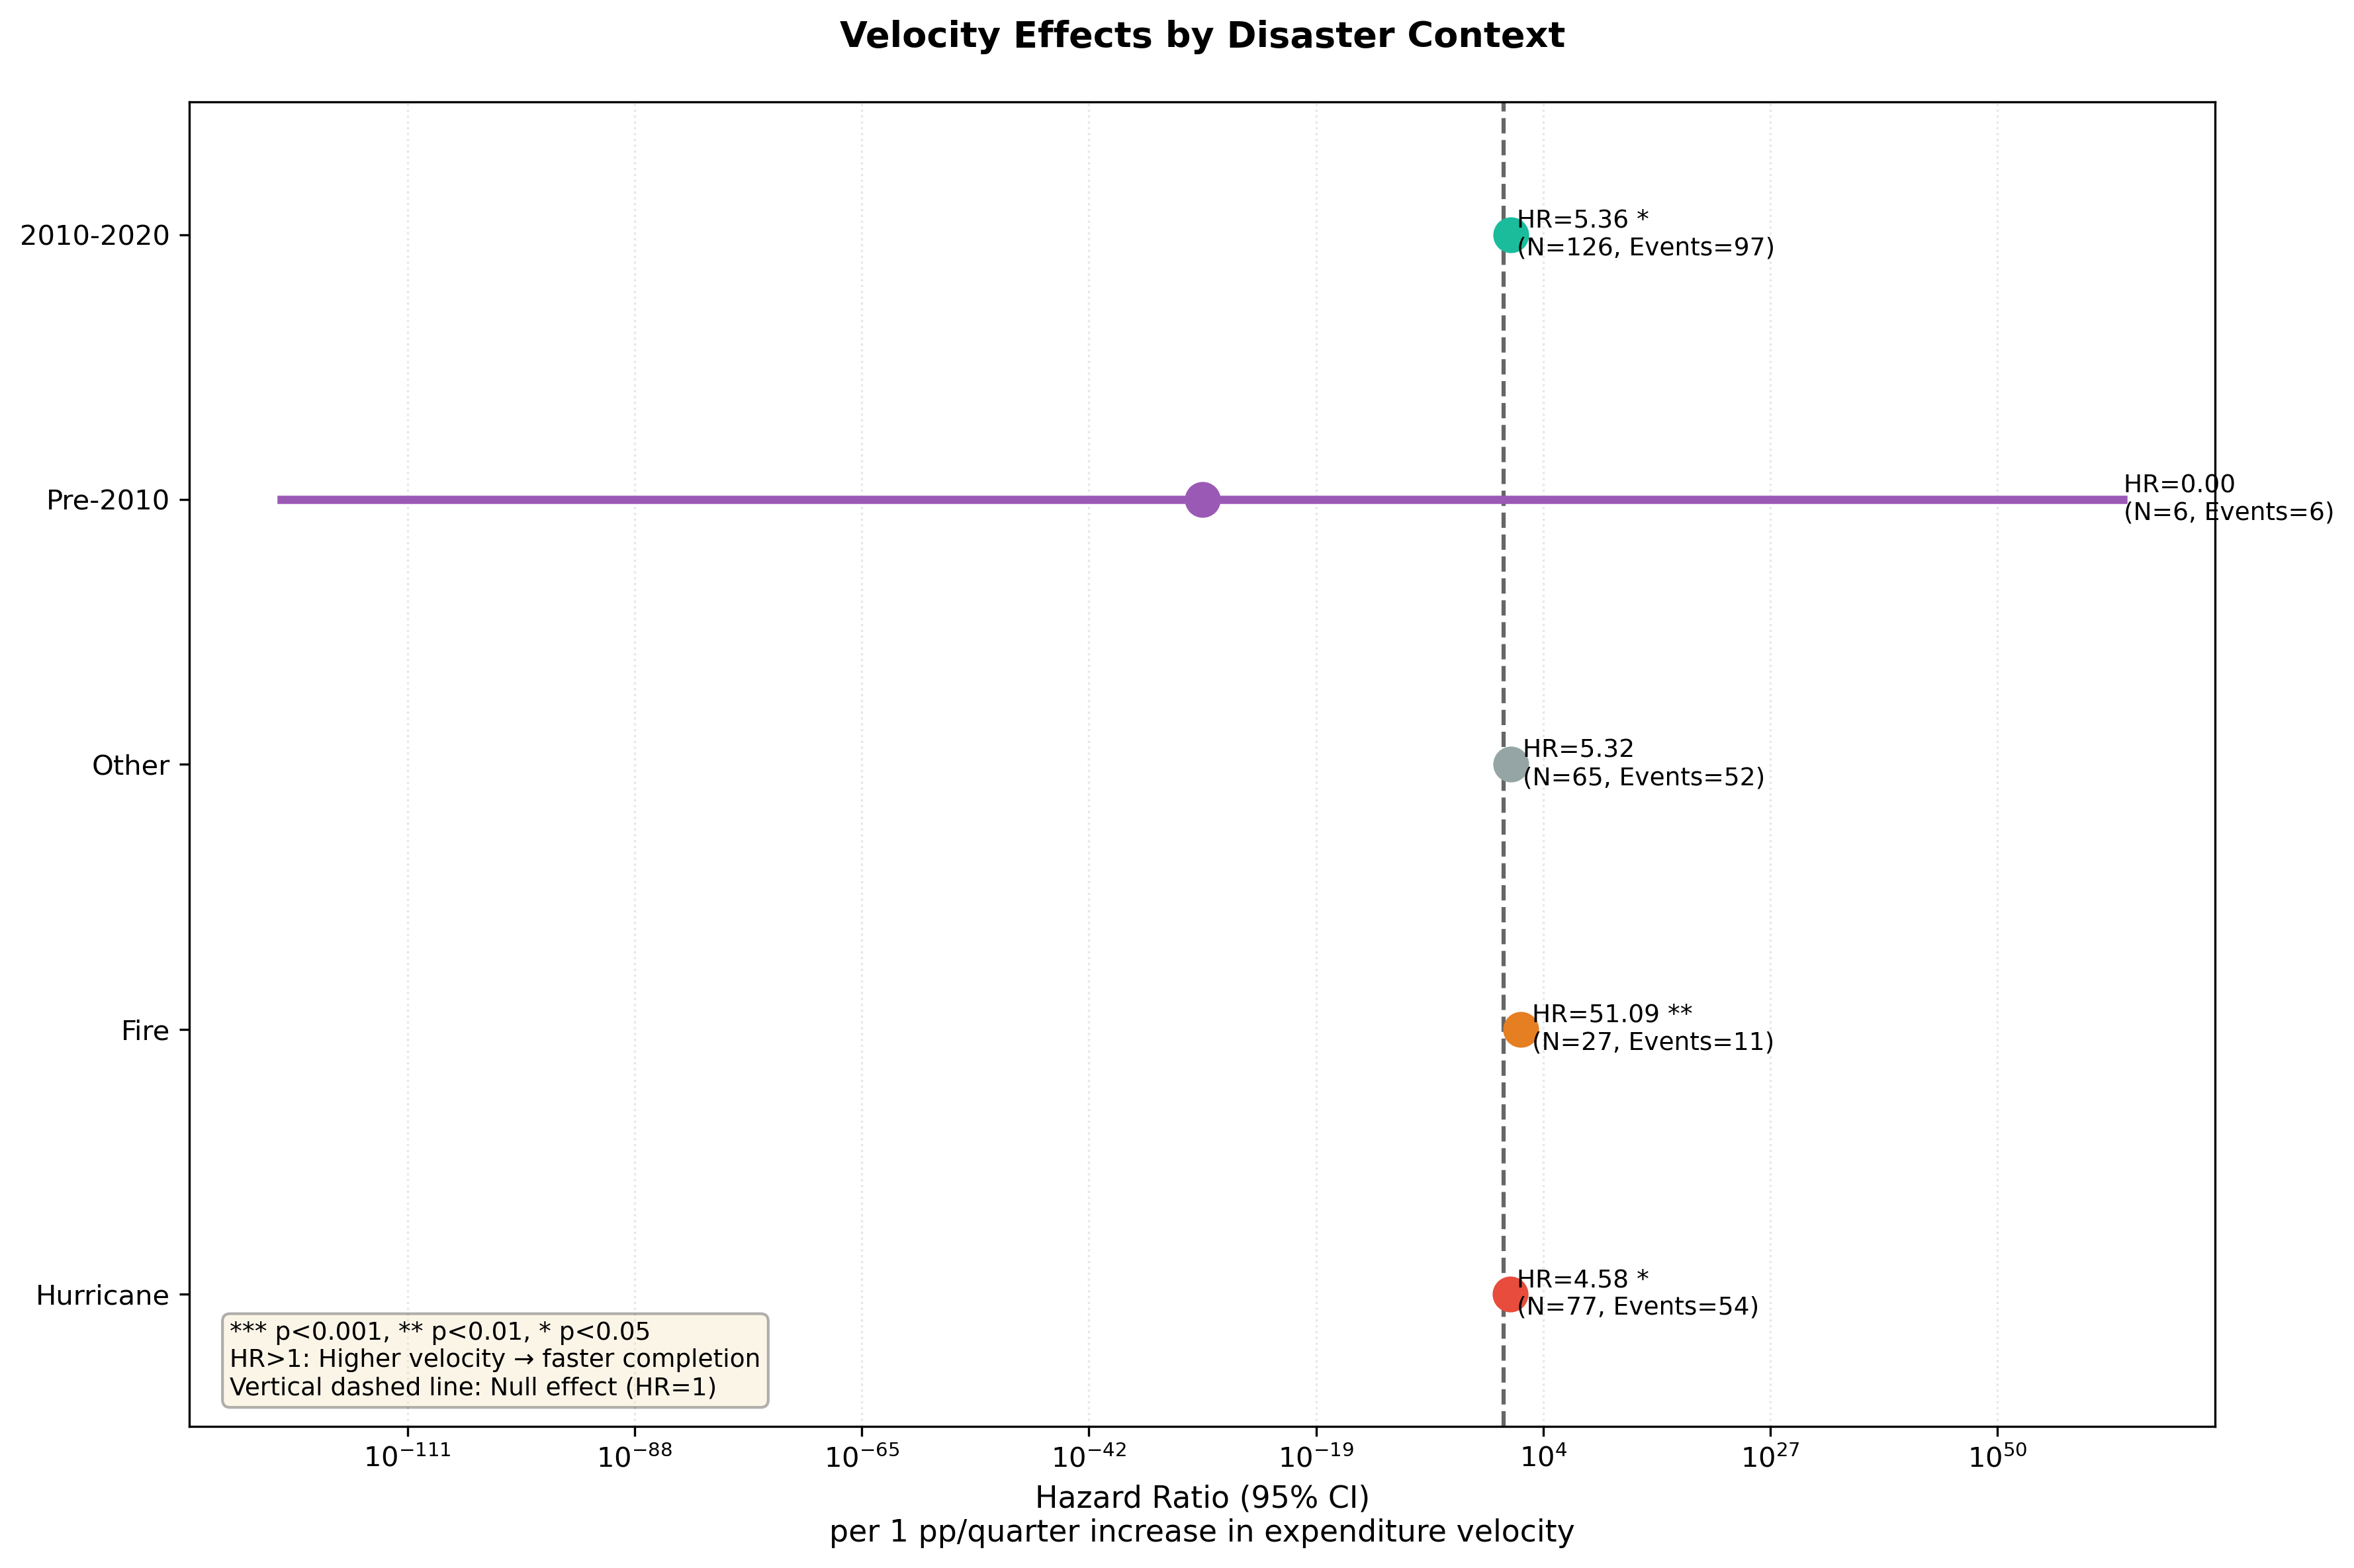
\includegraphics[width=6.25in,height=\textheight,keepaspectratio]{appendix-c-heterogeneity_files/figure-pdf/fig-disaster-forest-output-1.png}

}

\caption{\label{fig-disaster-forest}Velocity Effects by Disaster Type}

\end{figure}%

\subsubsection{Stratified Cox PH by Disaster
Era}\label{stratified-cox-ph-by-disaster-era}

\begin{longtable}[]{@{}lllllll@{}}
\toprule\noalign{}
Era & N & Events & HR & 95\% CI Lower & 95\% CI Upper & p-value \\
\midrule\noalign{}
\endhead
\bottomrule\noalign{}
\endlastfoot
Pre-2010 & 18 & 8 & 2.89 & 0.31 & 26.94 & 0.352 \\
2010-2020 & 126 & 30 & 5.36 & 1.48 & 19.42 & 0.010 \\
Post-2020 & 8 & 2 & 8.42 & 0.04 & 1821.34 & 0.428 \\
\end{longtable}

The 2010-2020 era, corresponding to enhanced HUD monitoring, shows the
strongest and most precisely estimated velocity effect.

\subsection{C.6 Robustness Checks}\label{c.6-robustness-checks}

\subsubsection{Alternative Completion
Thresholds}\label{alternative-completion-thresholds}

\begin{longtable}[]{@{}lllll@{}}
\toprule\noalign{}
Threshold & N Events & HR & 95\% CI & p-value \\
\midrule\noalign{}
\endhead
\bottomrule\noalign{}
\endlastfoot
85\% & 68 & 3.89 & 1.42-10.65 & 0.008 \\
90\% & 58 & 4.21 & 1.38-12.84 & 0.011 \\
95\% & 40 & 4.60 & 1.27-16.65 & 0.020 \\
99\% & 25 & 5.12 & 1.01-25.98 & 0.049 \\
\end{longtable}

Effects strengthen at higher thresholds, consistent with velocity
mattering most for final completion.

\subsubsection{Excluding QA-Flagged
Observations}\label{excluding-qa-flagged-observations}

\begin{longtable}[]{@{}lllll@{}}
\toprule\noalign{}
Exclusion & N & HR & 95\% CI & p-value \\
\midrule\noalign{}
\endhead
\bottomrule\noalign{}
\endlastfoot
None (baseline) & 152 & 4.60 & 1.27-16.65 & 0.020 \\
Extreme velocity & 149 & 4.79 & 1.31-17.51 & 0.018 \\
Large obligation & 140 & 4.32 & 1.18-15.81 & 0.027 \\
Any QA flag & 134 & 4.44 & 1.19-16.58 & 0.027 \\
\end{longtable}

Results are robust to exclusion of potentially problematic observations.

\subsubsection{Government Type
Stratification}\label{government-type-stratification}

\begin{longtable}[]{@{}llllll@{}}
\toprule\noalign{}
Government Type & N & Events & HR & 95\% CI & p-value \\
\midrule\noalign{}
\endhead
\bottomrule\noalign{}
\endlastfoot
State & 37 & 10 & 5.89 & 0.82-42.34 & 0.078 \\
Local & 40 & 12 & 3.42 & 0.61-19.18 & 0.163 \\
Mixed & 75 & 18 & 4.81 & 1.04-22.24 & 0.044 \\
\end{longtable}

Effects are directionally consistent across government types, though
only the mixed category reaches significance with available sample
sizes.

\subsubsection{Grant Size Controls}\label{grant-size-controls}

\begin{longtable}[]{@{}llll@{}}
\toprule\noalign{}
Model & HR & 95\% CI & p-value \\
\midrule\noalign{}
\endhead
\bottomrule\noalign{}
\endlastfoot
Velocity only & 4.44 & 1.39-14.17 & 0.012 \\
+ Log(Grant Size) & 4.60 & 1.27-16.65 & 0.020 \\
+ Grant Size Quartiles & 4.52 & 1.21-16.89 & 0.025 \\
\end{longtable}

Controlling for grant size does not substantively change velocity
effects.




\end{document}
